\documentclass[tikz, preview]{standalone}

\usepackage{amsfonts, amsthm, amssymb, amsmath, stmaryrd, etoolbox}
\usepackage{tikz}
\usetikzlibrary{matrix,arrows}

\begin{document}
\[
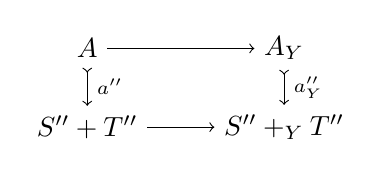
\begin{tikzpicture}
\node (BC) at (0,1) {$A$};
\node (BAC) at (2.5,1) {$A_Y$};
\node (BC') at (0,0) {$S''+T''$};
\node (BAC') at (2.5,0) {$S''+_YT''$};
%
\draw [->] (BC) edge (BAC);
\draw [font=\scriptsize,>->] (BC) edge node[right] {$a''$} (BC');
\draw [font=\scriptsize,>->] (BAC) edge node[right] {$a''_Y$} (BAC');
\draw [->] (BC') edge (BAC');
\end{tikzpicture}
\]
\end{document}
